
%% bare_conf.tex
%% V1.4a
%% 2014/09/17
%% by Michael Shell
%% See:
%% http://www.michaelshell.org/
%% for current contact information.
%%
%% This is a skeleton file demonstrating the use of IEEEtran.cls
%% (requires IEEEtran.cls version 1.8a or later) with an IEEE
%% conference paper.
%%
%% Support sites:
%% http://www.michaelshell.org/tex/ieeetran/
%% http://www.ctan.org/tex-archive/macros/latex/contrib/IEEEtran/
%% and
%% http://www.ieee.org/

%%*************************************************************************
%% Legal Notice:
%% This code is offered as-is without any warranty either expressed or
%% implied; without even the implied warranty of MERCHANTABILITY or
%% FITNESS FOR A PARTICULAR PURPOSE! 
%% User assumes all risk.
%% In no event shall IEEE or any contributor to this code be liable for
%% any damages or losses, including, but not limited to, incidental,
%% consequential, or any other damages, resulting from the use or misuse
%% of any information contained here.
%%
%% All comments are the opinions of their respective authors and are not
%% necessarily endorsed by the IEEE.
%%
%% This work is distributed under the LaTeX Project Public License (LPPL)
%% ( http://www.latex-project.org/ ) version 1.3, and may be freely used,
%% distributed and modified. A copy of the LPPL, version 1.3, is included
%% in the base LaTeX documentation of all distributions of LaTeX released
%% 2003/12/01 or later.
%% Retain all contribution notices and credits.
%% ** Modified files should be clearly indicated as such, including  **
%% ** renaming them and changing author support contact information. **
%%
%% File list of work: IEEEtran.cls, IEEEtran_HOWTO.pdf, bare_adv.tex,
%%                    bare_conf.tex, bare_jrnl.tex, bare_conf_compsoc.tex,
%%                    bare_jrnl_compsoc.tex, bare_jrnl_transmag.tex
%%*************************************************************************


% *** Authors should verify (and, if needed, correct) their LaTeX system  ***
% *** with the testflow diagnostic prior to trusting their LaTeX platform ***
% *** with production work. IEEE's font choices and paper sizes can       ***
% *** trigger bugs that do not appear when using other class files.       ***                          ***
% The testflow support page is at:
% http://www.michaelshell.org/tex/testflow/



\documentclass[conference]{IEEEtran}
% Some Computer Society conferences also require the compsoc mode option,
% but others use the standard conference format.
%
% If IEEEtran.cls has not been installed into the LaTeX system files,
% manually specify the path to it like:
% \documentclass[conference]{../sty/IEEEtran}





% Some very useful LaTeX packages include:
% (uncomment the ones you want to load)


% *** MISC UTILITY PACKAGES ***
%
%\usepackage{ifpdf}
% Heiko Oberdiek's ifpdf.sty is very useful if you need conditional
% compilation based on whether the output is pdf or dvi.
% usage:
% \ifpdf
%   % pdf code
% \else
%   % dvi code
% \fi
% The latest version of ifpdf.sty can be obtained from:
% http://www.ctan.org/tex-archive/macros/latex/contrib/oberdiek/
% Also, note that IEEEtran.cls V1.7 and later provides a builtin
% \ifCLASSINFOpdf conditional that works the same way.
% When switching from latex to pdflatex and vice-versa, the compiler may
% have to be run twice to clear warning/error messages.

\usepackage{graphicx}

\usepackage{algorithm}
\usepackage{algpseudocode}
\usepackage{amsmath}
\usepackage{amssymb}
\usepackage{amsthm}
\usepackage{etoolbox}
\usepackage{changepage}
\usepackage{csquotes}
\usepackage{tabularx,booktabs,multirow}
\usepackage{longtable}
\usepackage{framed}

\graphicspath{{Graphics/}}

\newcommand{\sym}[1]{\ensuremath{\mathcal{#1}}}
\newcommand{\obj}[1]{\ensuremath{#1}}

\newtheorem{definition}{Definition}
\newtheorem{question}{Question}
\AfterEndEnvironment{definition}{\noindent\ignorespaces}

\theoremstyle{definition}
\newtheorem{example}{Example}
\newtheorem{experiment}{Experiment}[question]
\newtheorem{observation}{Observation}[question]
%\AfterEndEnvironment{example}{\noindent\ignorespaces}

\newcommand{\svm}{SVM$^{rank}$}
\newcommand{\cen}[1]{
  \begin{center}
    #1
  \end{center}
}

\newenvironment{demo}{\begin{adjustwidth}{2cm}{}}{\end{adjustwidth}}

\makeatletter
\newenvironment{shiftedflalign}{%
    \start@align\tw@\st@rredfalse\m@ne%
    \hskip\parindent
}{%
    \endalign
}
\newenvironment{shiftedflalign*}{%
    \start@align\tw@\st@rredtrue\m@ne
    \hskip\parindent
}{%
    \endalign
}
\makeatother

\newcommand{\tabspace}{\  \  \  \  }


% *** CITATION PACKAGES ***
%
%\usepackage{cite}
% cite.sty was written by Donald Arseneau
% V1.6 and later of IEEEtran pre-defines the format of the cite.sty package
% \cite{} output to follow that of IEEE. Loading the cite package will
% result in citation numbers being automatically sorted and properly
% "compressed/ranged". e.g., [1], [9], [2], [7], [5], [6] without using
% cite.sty will become [1], [2], [5]--[7], [9] using cite.sty. cite.sty's
% \cite will automatically add leading space, if needed. Use cite.sty's
% noadjust option (cite.sty V3.8 and later) if you want to turn this off
% such as if a citation ever needs to be enclosed in parenthesis.
% cite.sty is already installed on most LaTeX systems. Be sure and use
% version 5.0 (2009-03-20) and later if using hyperref.sty.
% The latest version can be obtained at:
% http://www.ctan.org/tex-archive/macros/latex/contrib/cite/
% The documentation is contained in the cite.sty file itself.






% *** GRAPHICS RELATED PACKAGES ***
%
\ifCLASSINFOpdf
  % \usepackage[pdftex]{graphicx}
  % declare the path(s) where your graphic files are
  % \graphicspath{{../pdf/}{../jpeg/}}
  % and their extensions so you won't have to specify these with
  % every instance of \includegraphics
  % \DeclareGraphicsExtensions{.pdf,.jpeg,.png}
\else
  % or other class option (dvipsone, dvipdf, if not using dvips). graphicx
  % will default to the driver specified in the system graphics.cfg if no
  % driver is specified.
  % \usepackage[dvips]{graphicx}
  % declare the path(s) where your graphic files are
  % \graphicspath{{../eps/}}
  % and their extensions so you won't have to specify these with
  % every instance of \includegraphics
  % \DeclareGraphicsExtensions{.eps}
\fi
% graphicx was written by David Carlisle and Sebastian Rahtz. It is
% required if you want graphics, photos, etc. graphicx.sty is already
% installed on most LaTeX systems. The latest version and documentation
% can be obtained at: 
% http://www.ctan.org/tex-archive/macros/latex/required/graphics/
% Another good source of documentation is "Using Imported Graphics in
% LaTeX2e" by Keith Reckdahl which can be found at:
% http://www.ctan.org/tex-archive/info/epslatex/
%
% latex, and pdflatex in dvi mode, support graphics in encapsulated
% postscript (.eps) format. pdflatex in pdf mode supports graphics
% in .pdf, .jpeg, .png and .mps (metapost) formats. Users should ensure
% that all non-photo figures use a vector format (.eps, .pdf, .mps) and
% not a bitmapped formats (.jpeg, .png). IEEE frowns on bitmapped formats
% which can result in "jaggedy"/blurry rendering of lines and letters as
% well as large increases in file sizes.
%
% You can find documentation about the pdfTeX application at:
% http://www.tug.org/applications/pdftex





% *** MATH PACKAGES ***
%
%\usepackage[cmex10]{amsmath}
% A popular package from the American Mathematical Society that provides
% many useful and powerful commands for dealing with mathematics. If using
% it, be sure to load this package with the cmex10 option to ensure that
% only type 1 fonts will utilized at all point sizes. Without this option,
% it is possible that some math symbols, particularly those within
% footnotes, will be rendered in bitmap form which will result in a
% document that can not be IEEE Xplore compliant!
%
% Also, note that the amsmath package sets \interdisplaylinepenalty to 10000
% thus preventing page breaks from occurring within multiline equations. Use:
%\interdisplaylinepenalty=2500
% after loading amsmath to restore such page breaks as IEEEtran.cls normally
% does. amsmath.sty is already installed on most LaTeX systems. The latest
% version and documentation can be obtained at:
% http://www.ctan.org/tex-archive/macros/latex/required/amslatex/math/





% *** SPECIALIZED LIST PACKAGES ***
%
%\usepackage{algorithmic}
% algorithmic.sty was written by Peter Williams and Rogerio Brito.
% This package provides an algorithmic environment fo describing algorithms.
% You can use the algorithmic environment in-text or within a figure
% environment to provide for a floating algorithm. Do NOT use the algorithm
% floating environment provided by algorithm.sty (by the same authors) or
% algorithm2e.sty (by Christophe Fiorio) as IEEE does not use dedicated
% algorithm float types and packages that provide these will not provide
% correct IEEE style captions. The latest version and documentation of
% algorithmic.sty can be obtained at:
% http://www.ctan.org/tex-archive/macros/latex/contrib/algorithms/
% There is also a support site at:
% http://algorithms.berlios.de/index.html
% Also of interest may be the (relatively newer and more customizable)
% algorithmicx.sty package by Szasz Janos:
% http://www.ctan.org/tex-archive/macros/latex/contrib/algorithmicx/




% *** ALIGNMENT PACKAGES ***
%
%\usepackage{array}
% Frank Mittelbach's and David Carlisle's array.sty patches and improves
% the standard LaTeX2e array and tabular environments to provide better
% appearance and additional user controls. As the default LaTeX2e table
% generation code is lacking to the point of almost being broken with
% respect to the quality of the end results, all users are strongly
% advised to use an enhanced (at the very least that provided by array.sty)
% set of table tools. array.sty is already installed on most systems. The
% latest version and documentation can be obtained at:
% http://www.ctan.org/tex-archive/macros/latex/required/tools/


% IEEEtran contains the IEEEeqnarray family of commands that can be used to
% generate multiline equations as well as matrices, tables, etc., of high
% quality.




% *** SUBFIGURE PACKAGES ***
%\ifCLASSOPTIONcompsoc
%  \usepackage[caption=false,font=normalsize,labelfont=sf,textfont=sf]{subfig}
%\else
%  \usepackage[caption=false,font=footnotesize]{subfig}
%\fi
% subfig.sty, written by Steven Douglas Cochran, is the modern replacement
% for subfigure.sty, the latter of which is no longer maintained and is
% incompatible with some LaTeX packages including fixltx2e. However,
% subfig.sty requires and automatically loads Axel Sommerfeldt's caption.sty
% which will override IEEEtran.cls' handling of captions and this will result
% in non-IEEE style figure/table captions. To prevent this problem, be sure
% and invoke subfig.sty's "caption=false" package option (available since
% subfig.sty version 1.3, 2005/06/28) as this is will preserve IEEEtran.cls
% handling of captions.
% Note that the Computer Society format requires a larger sans serif font
% than the serif footnote size font used in traditional IEEE formatting
% and thus the need to invoke different subfig.sty package options depending
% on whether compsoc mode has been enabled.
%
% The latest version and documentation of subfig.sty can be obtained at:
% http://www.ctan.org/tex-archive/macros/latex/contrib/subfig/




% *** FLOAT PACKAGES ***
%
%\usepackage{fixltx2e}
% fixltx2e, the successor to the earlier fix2col.sty, was written by
% Frank Mittelbach and David Carlisle. This package corrects a few problems
% in the LaTeX2e kernel, the most notable of which is that in current
% LaTeX2e releases, the ordering of single and double column floats is not
% guaranteed to be preserved. Thus, an unpatched LaTeX2e can allow a
% single column figure to be placed prior to an earlier double column
% figure. The latest version and documentation can be found at:
% http://www.ctan.org/tex-archive/macros/latex/base/


%\usepackage{stfloats}
% stfloats.sty was written by Sigitas Tolusis. This package gives LaTeX2e
% the ability to do double column floats at the bottom of the page as well
% as the top. (e.g., "\begin{figure*}[!b]" is not normally possible in
% LaTeX2e). It also provides a command:
%\fnbelowfloat
% to enable the placement of footnotes below bottom floats (the standard
% LaTeX2e kernel puts them above bottom floats). This is an invasive package
% which rewrites many portions of the LaTeX2e float routines. It may not work
% with other packages that modify the LaTeX2e float routines. The latest
% version and documentation can be obtained at:
% http://www.ctan.org/tex-archive/macros/latex/contrib/sttools/
% Do not use the stfloats baselinefloat ability as IEEE does not allow
% \baselineskip to stretch. Authors submitting work to the IEEE should note
% that IEEE rarely uses double column equations and that authors should try
% to avoid such use. Do not be tempted to use the cuted.sty or midfloat.sty
% packages (also by Sigitas Tolusis) as IEEE does not format its papers in
% such ways.
% Do not attempt to use stfloats with fixltx2e as they are incompatible.
% Instead, use Morten Hogholm'a dblfloatfix which combines the features
% of both fixltx2e and stfloats:
%
% \usepackage{dblfloatfix}
% The latest version can be found at:
% http://www.ctan.org/tex-archive/macros/latex/contrib/dblfloatfix/




% *** PDF, URL AND HYPERLINK PACKAGES ***
%
%\usepackage{url}
% url.sty was written by Donald Arseneau. It provides better support for
% handling and breaking URLs. url.sty is already installed on most LaTeX
% systems. The latest version and documentation can be obtained at:
% http://www.ctan.org/tex-archive/macros/latex/contrib/url/
% Basically, \url{my_url_here}.




% *** Do not adjust lengths that control margins, column widths, etc. ***
% *** Do not use packages that alter fonts (such as pslatex).         ***
% There should be no need to do such things with IEEEtran.cls V1.6 and later.
% (Unless specifically asked to do so by the journal or conference you plan
% to submit to, of course. )


% correct bad hyphenation here
\hyphenation{op-tical net-works semi-conduc-tor nauw-keu-rig-heid pre-di-ca-ten ont-wik-keld be-schrij-ven}


\begin{document}
%
% paper title
% Titles are generally capitalized except for words such as a, an, and, as,
% at, but, by, for, in, nor, of, on, or, the, to and up, which are usually
% not capitalized unless they are the first or last word of the title.
% Linebreaks \\ can be used within to get better formatting as desired.
% Do not put math or special symbols in the title.
\title{Het leren van beperkingen en optimalisatie criteria}


% author names and affiliations
% use a multiple column layout for up to three different
% affiliations
\author{\IEEEauthorblockN{Samuel Kolb}
\IEEEauthorblockA{Departement Computerwetenschappen\\
Katholieke Universiteit Leuven\\
Leuven, Belgi\"e\\
Email: samuel.kolb@me.com}}

% conference papers do not typically use \thanks and this command
% is locked out in conference mode. If really needed, such as for
% the acknowledgment of grants, issue a \IEEEoverridecommandlockouts
% after \documentclass

% for over three affiliations, or if they all won't fit within the width
% of the page, use this alternative format:
% 
%\author{\IEEEauthorblockN{Michael Shell\IEEEauthorrefmark{1},
%Homer Simpson\IEEEauthorrefmark{2},
%James Kirk\IEEEauthorrefmark{3}, 
%Montgomery Scott\IEEEauthorrefmark{3} and
%Eldon Tyrell\IEEEauthorrefmark{4}}
%\IEEEauthorblockA{\IEEEauthorrefmark{1}School of Electrical and Computer Engineering\\
%Georgia Institute of Technology,
%Atlanta, Georgia 30332--0250\\ Email: see http://www.michaelshell.org/contact.html}
%\IEEEauthorblockA{\IEEEauthorrefmark{2}Twentieth Century Fox, Springfield, USA\\
%Email: homer@thesimpsons.com}
%\IEEEauthorblockA{\IEEEauthorrefmark{3}Starfleet Academy, San Francisco, California 96678-2391\\
%Telephone: (800) 555--1212, Fax: (888) 555--1212}
%\IEEEauthorblockA{\IEEEauthorrefmark{4}Tyrell Inc., 123 Replicant Street, Los Angeles, California 90210--4321}}




% use for special paper notices
%\IEEEspecialpapernotice{(Invited Paper)}




% make the title area
\maketitle

% As a general rule, do not put math, special symbols or citations
% in the abstract
\begin{abstract}
Deze paper presenteert een leersysteem voor beperkingen en een leersysteem voor optimalisatie criteria.
Beperking worden geleerd in de vorm van clausules in eerste orde logica door het gebruik van ILP technieken.
Voor de optimalisatie criteria wordt het gebruik van gewogen clausules voorgesteld.
Beide systemen zijn in staat om essenti\"ele beperkingen en optimalisatie criteria te leren.
De invloed van verschillende interne en externe factoren wordt onderzocht.
Er wordt een procedure voorgesteld om de gewogen clausules in eerste orde logica te gebruiken om optimale oplossingen te vinden.
\end{abstract}

% no keywords




% For peer review papers, you can put extra information on the cover
% page as needed:
% \ifCLASSOPTIONpeerreview
% \begin{center} \bfseries EDICS Category: 3-BBND \end{center}
% \fi
%
% For peerreview papers, this IEEEtran command inserts a page break and
% creates the second title. It will be ignored for other modes.
\IEEEpeerreviewmaketitle

%!TEX root=Paper.tex
\section{Introductie}
% no \IEEEPARstart
% You must have at least 2 lines in the paragraph with the drop letter
% (should never be an issue)

Computers worden veelal gebruikt voor het oplossen van problemen die handmatig maar moeilijk opgelost kunnen worden. 
Hiervoor worden klassiek computerprogramma's gebruikt.
Dit zijn essentieel stap-voor-stap instructies die beschrijven hoe een probleem opgelost moet worden.
Als alternatief voor dit soort \emph{imperatief} programmeren kunnen problemen beschreven worden op een \emph{declaratieve} manier.
Hierbij ligt de focus op het formuleren van het probleem op een hoog niveau.
Zo een taal beschrijft het probleem zonder in te vullen hoe een oplossing gevonden moet worden.
Voor deze talen worden generische algoritmes ontworpen die automatisch oplossingen kunnen zoeken.

Een populaire stroming binnen het veld van declaratief programmeren is constraint programming.
In constraint programming worden variabelen gebruikt om problemen voor te stellen.
Elke variabele heeft een domein en er worden beperkingen (constraints) opgelegd aan de waarden van de variabelen.
De constraint solver zal proberen elke variabele een waarde uit zijn domein toe te kennen zodanig dat alle beperkingen voldaan zijn.
Hierbij focust de gebruiker op het opstellen van de beperkingen en kan de solver zelf kiezen op welke manier oplossingen gevonden kunnen worden.

Constraint programming is niet enkel populair binnen de academische wereld, het wordt ook succesvol gebruikt in de industrie\cite{Simonis:IndustrialApplicationsCP}.
De meeste aandacht wordt besteed aan het verbeteren van solvers, maar het blijkt in de praktijk best moeilijk voor niet-deskundigen om beperkingen te formuleren\cite{Wallace:PrinciplesCP}.

Het eerste doel van dit onderzoek is het automatiseren van het opstellen van beperkingen.
Door deze beperkingen te leren met behulp van enkele voorbeelden, probeert dit werk om onder andere het programmeren met beperkingen toegankelijker te maken.

Beperkingen zullen worden uitgedrukt door logische clausules (clauses).
Deze laten toe om technieken uit het veld van inductief logisch programmeren (ILP) te gebruiken.
Specifiek, wordt een nieuwe implementatie van het clausal discovery algoritme\cite{DeRaedt:ClausalDiscovery} uitgewerkt.
Onderzoek naar technieken voor het leren van beperkingen loopt vaak onafhankelijk van de ontwikkelingen in ILP.
Dit onderzoek knoopt aan bij het idee van Lallouet et al.\cite{Lallouet:LearningCP} om voor deze taak ILP technieken te gebruiken.
\\\\
Harde beperkingen kunnen gebruikt worden om oplossingen te onderscheiden van niet-oplossingen.
Zogenaamde zachte beperkingen (soft constraints) kunnen eigenschappen uitdrukken die niet voldaan hoeven te zijn.
Door aan zulke beperkingen gewichten te geven kan het belang van dergelijke beperkingen uitgedrukt worden.
Dit laat toe om binnen de toelaatbare oplossingen een optimale oplossing te vinden.
Deze oplossing voldoet aan zo veel mogelijk belangrijke beperkingen.

Het tweede doel van dit onderzoek omvat het leren van de voorkeuren van een gebruiker en het formuleren van overeenkomstige optimalisatie criteria.
Door middel van rangschikkingen van een aantal voorbeelden worden gewogen zachte beperkingen opgesteld.
Dit moet, zoals het leren van beperkingen, de kloof tussen problemen en formele representaties verkleinen.

Het gebruik van gewogen zachte beperkingen is onder andere ge\"inspireerd door het onderzoek van Campigotto et al.\cite{campigotto2011active}.
Hierin wordt een gelijkaardige doelstelling onderzocht in een interactieve context voor propositionele beperkingen.
In dit onderzoek zullen beperkingen in eerste orde logica worden gebruikt.
\\\\
Het volledige proces van probleem naar oplossing vergt ook een solver voor het automatisch vinden van een oplossing.
Voor de gewogen beperkingen die door dit systeem geleerd worden bestaat er geen solver die deze representatie direct kan gebruiken.
Daarom zal worden aangetoond hoe deze beperkingen in de praktijk gebruikt kunnen worden om een optimale oplossing te vinden.

% ----------------------------------------
% Achtergrond
% ----------------------------------------

\section{Achtergrond}
Deze sectie geeft een bondig overzicht over gebuikte concepten en relevante literatuur.

\subsection{Clausules}
Clausules in eerste orde logica zijn disjuncties van literalen.
Een literaal is gedefinieerd als een atoom of de negatie van een atoom.
Vaak worden clausules uitgedrukt door middel van een lichaam (body) en hoofd (head): $\mathit{hoofd} \leftarrow \mathit{lichaam}$.
Alle literalen met een negatie worden gegroepeerd in het lichaam en en de anderen in het hoofd.
\begin{align*}
  \lnot a_1 \lor \lnot a_2 \lor a_3 \lor a_4 = a_3, a_4 \leftarrow a_1, a_2 
\end{align*}

Atomen zijn logische concepten waaraan een waarheidswaarde kan worden toegekend.
In dit onderzoek zijn atomen beperkt tot predicaten.
Een predicaat bevat een predicaat symbool en een aantal termen.
Die termen zijn constanten of variabelen en beschrijven objecten in een domein.
Predicaten drukken relaties uit tussen die objecten: $\mathit{symbool}(\mathit{term_1}, ... \mathit{term_n})$.
De clausules die in dit onderzoek geleerd worden bevatten enkel variabelen.

\subsection{Leren van beperkingen}
Het leren van beperkingen is een moeilijk probleem.
De zoekruimte om beperkingen te vinden is vaak erg groot.
Bovendien zijn er, in tegenstelling tot veel problemen binnen het veld van machinaal leren, meestal weinig voorbeelden gegeven om van te leren.

Verschillende systemen proberen het leren van beperkingen op verschillende manieren op te lossen.
Een manier om het probleem van weinig data op te lossen is om data interactief te genereren.
De systemen Conacq2\cite{bessiere2007query} en QuAck\cite{bessiere2013constraint} genereren voorbeelden en vragen aan de gebruiker om deze al dan niet goed te keuren.

In een passieve setting probeert ModelSeeker\cite{Beldiceanu:ModelSeeker} de probleem variabelen op verschillende manieren te structureren.
Daaraan wordt getest of dat bepaalde algemene beperkingen gelden binnen deze structuren.
Deze manier laat toe om effici\"ent beperkingen te leren van maar enkele voorbeelden.

Zoals vermeld werd in de inleiding werd in het onderzoek van Lallouet et al.\cite{Lallouet:LearningCP} ook al geprobeerd om ILP technieken te gebruiken voor het leren van beperkingen.
Hierbij wordt de zoekruimte van mogelijke beperkingen op een bidirectionele manier doorzocht waarbij vooral negatieve voorbeelden gebruikt worden.

\begin{algorithm}
  \caption{Clausal discovery algoritme}
  \label{alg:cd_alg}

  \begin{algorithmic}
  \State $\sym{D} \gets Examples$
  \State $Q \gets \{\square\}$
  \State $\sym{T} \gets \{\}$
  \While{$\lnot isempty(Q)$}
    \State $c \gets next(Q)$
    \If{$covers(c, \sym{D})$}
      \If{$\lnot entails(\sym{T}, c)$}
        \State $\sym{T} = \sym{T} \cup c$
      \EndIf
    \Else
      \State $Q \gets Q \cup \rho(c)$
    \EndIf
  \EndWhile
  \State $\sym{T} \gets prune(\sym{T})$
  \State \Return \sym{T}
\end{algorithmic}
\end{algorithm}

In dit onderzoek werd er vooral gekeken naar clausal discovery\cite{DeRaedt:ClausalDiscovery}.
Het algoritme~\ref{alg:cd_alg} werd voorgesteld om vooral op basis van positieve voorbeelden logische clausules te leren.
Dit algoritme bevat bepaalde conceptuele functies zoals $\mathit{covers}, \mathit{entails}$ en $\rho$.
Het systeem dat in dit onderzoek ontwikkeld werd gebruikt deze functies maar vult deze anders in.
Om te berekenen of een clausule waar is voor de voorbeelden in een dataset ($\mathit{covers}$) en of een nieuwe clausule een logisch gevolg is van de reeds gevonden clausules ($\mathit{entails}$) wordt een logisch systeem gebruikt.
De functie $\rho$ wordt de \textit{refinement operator} genoemd.
Deze produceert verschillende mogelijke uitbreidingen van een clausule.
Elke uitbreiding wordt verkregen door een literaal toe te voegen aan de gegeven clausule.
Zodanig wordt, vertrekkende van de lege clausule~($\square$), de zoekruimte verkend door clausules steeds algemener te maken.

\subsection{Logische solver}
Dit onderzoek gebruikt het logisch systeem IDP\cite{de2013prototype,wittocx2008idp} om de functies $\mathit{convers}$ en $\mathit{entails}$ te berekenen.
Het systeem laat toe om oplossingen te verifi\"eren maar ook te genereren.
IDP ondersteunt een uitbreiding van eerste orde logica: $FO(\cdot)$.
Achtergrondkennis van een gebruiker over de gebruikte predicaten kan in dit formaat worden meegegeven.

\subsection{Optimalisatie}
De vraag of er aan een propositionele logische formule voldaan kan worden wordt het vervulbaarheidsprobleem (SAT) genoemd.
Een uitbreiding hiervan is het MAX-SAT probleem.
Hierin wordt geprobeerd om in een formule in conjunctieve normaalvorm (CNF) zoveel mogelijk clausules (disjuncties) waar te maken.
Als aan die clauses een gewicht wordt toegekend bekomt men het gewogen MAX-SAT probleem.
In Campigotto et al.\cite{campigotto2011active} werd het automatische leren van propositionele formules en gewichten onderzocht.
Ge\"inspireerd door hun resultaten zullen in dit onderzoek eerste orde logische optimalisatie criteria gezocht worden.
Het optimalisatie vraagstuk kan dan gezien worden als een uitbreiding van gewogen MAX-SAT waarbij de clausules in eerste orde logica zijn.

% ----------------------------------------
% Probleemstelling
% ----------------------------------------

\section{Probleemstelling}
Dit onderzoekt heeft hoofdzakelijk twee doelen: het leren van beperkingen en het leren van optimalisatie technieken.
De systemen die in de context van deze doelstellingen ontworpen worden proberen het opstellen van formele representaties te vereenvoudigen.
Om de software toegankelijk te maken wordt er aandacht besteed aan de informatie die van de gebruiker gevraagd wordt.

\begin{framed}
  \noindent
  \begin{minipage}{\textwidth}
    \paragraph*{Doel 1}
    Gegeven een aantal voorbeelden en een limiet $t$ is het doel van het leersysteem voor beperkingen om zo specifiek mogelijke clausules te vinden die door ten minste $t$ van de gegeven voorbeelden voldaan worden.
  \end{minipage}
\end{framed}

Voorbeelden beschrijven specifieke oplossingen.
Ze bevatten een set objecten en beschrijven exhaustief alle relaties (predicaten) die van toepassing zijn op deze objecten.
De geleerde clausules zijn onafhankelijk van de specifieke objecten in de voorbeelden en bevatten enkel variabelen.

\begin{framed}
  \noindent
  \begin{minipage}{\textwidth}
    \paragraph*{Doel 2}
    Gegeven een aantal voorbeelden en een aantal rangschikkingen over deze voorbeelden is het doel van het leersysteem voor optimalisatie criteria om zachte beperkingen en gewichten te vinden, zodanig dat de orde die door deze criteria beschreven wordt optimaal overeenkomt met de gegeven rangschikkingen.
  \end{minipage}
\end{framed}

De zachte beperkingen zijn clausules die op sommige van de voorbeelden gelden.
Rangschikkingen zijn van het formaat: $e_x = e_y > ... > e_a = e_b$ en beschrijven telkens een parti\"ele orde.
Door middel van de gewogen clausules kan voor elk voorbeeld een score berekend worden.
\begin{align*}
  \sum\limits_{\mathit{gewicht}, \mathit{c}} \mathit{gewicht} \cdot v_{c}
\end{align*}
Indien de clausule voldaan is voor het voorbeeld is de term $v_c = 1$, anders is $v_c = 0$.
Met behulp van deze scores kan een totale orde gedefinieerd worden over de voorbeelden.
\\\\
Een derde doel van deze thesis is om aan te tonen hoe deze beperkingen en vooral de optimalisatie criteria in de praktijk gebruikt kunnen worden om een optimale oplossing te vinden.

% ----------------------------------------
% Aanpak
% ----------------------------------------

\section{Aanpak}
Voor dit onderzoek werd een implementatie gecre\"eerd van een leersysteem voor clausules en een leersysteem voor gewogen clausules.
Figuur~\ref{fig:struktuur} toont een overzicht.
Clausules worden geleerd met behulp van voorbeelden.
Om gewogen clausules te vinden wordt eerst behulp gemaakt van het leersysteem van clausules om zachte beperkingen te vinden.
Daarna worden gewichten voor deze beperkingen bepaald op basis van de rangschikkingen.
Dit gebeurt met behulp van de \svm software.

\begin{figure}

  \centering
    \includegraphics[width=1\linewidth]{AanpakOverzicht.pdf}
  \caption{Overzicht aanpak}
  \label{fig:struktuur}

\end{figure}

\subsection{Formaat}
De voorbeelden worden gegroepeerd in een bestand.
In het begin van het bestand volgen een aantal definities van types en predicaten.
Types zijn een vorm van kennis die een gebruiker vaak heeft en die de nauwkeurigheid en effici\"entie van het systeem ten goede komt.
Definities van predicaten beschrijven wat voor types de termen van dat predicaat moeten hebben.
Twee speciale vormen van predicaten zijn toegelaten: berekende predicaten en symmetrische predicaten.
Voor berekende predicaten wordt in de achtergrondkennis gespecificeerd hoe ze berekend moeten worden.
Deze predicaten worden dus niet expliciet gegeven in de voorbeelden.
Symmetrische predicaten zijn predicaten waarbij de volgorde van de predicaten niet uitmaakt.

\subsection{Clausal discovery}
Het leersysteem voor clausules is, zoals eerder vernoemd, gebaseerd op clausal discovery.
Voor de essenti\"ele functies $\mathit{covers}$ en $\mathit{entails}$ wordt het logisch systeem IDP gebruikt.
IDP gebruikt vier componenten: een vocabularium van types en definities, theorie\"en van formules, structuren en een procedure.
Het vocabularium kan worden gegenereerd vanuit de definities en structuren.
Voorbeelden kunnen gezien worden als structuren, maar structuren moeten niet volledig gespecificeerd zijn.
De procedure wordt gebruikt om verschillende soorten inferenties uit te voeren over de theorie\"en en structuren.
Voorbeelden zijn het verifi\"eren of het het vervolledigen van een structuur gegeven een theorie.

Als een clausule in de wachtrij geplaatst wordt zullen de nodige IDP componenten gegenereerd worden om de $\mathit{covers}$ test uit te voeren.
Zodra de clausule uit de wachtrij genomen wordt, worden twee tests uitgevoerd.
De subset-test bepaalt of dat de clausule een super set is van een andere clausule die eerder al geaccepteerd werd.
Indien dat zo is en de andere clausule voor dezelfde voorbeelden geldt, dan is de nieuwe clausule onnodig.
Anders zal getest worden of dat de clausule zelf voor genoeg voorbeelden voldaan is.
Indien ja, zo wordt zij geaccepteerd en mogelijks als beperking aanvaard, anders wordt de clausule uitgebreid door $\rho$.
Een geaccepteerde clausule kan redundant zijn als ze een logisch gevolg is van de achtergrond kennis en de reeds gevonden beperkingen.
Dit wordt achterhaald door de $\mathit{entails}$ functie, gebruikmakende van IDP.

Een belangrijke stap is het uitbreiden van clausules.
Op basis van het maximum aantal variabelen wordt op voorhand een lijst~$L$ opgesteld van atomen die kunnen worden toegevoegd aan een clausule.
Binnen het lichaam en hoofd van de clausule mogen deze atomen enkel in de juiste volgorde worden toegevoegd.
Bovendien moet er voldaan worden aan de types van de predicaten en zijn er restricties op het formaat van de clausules.
Clausules moeten \emph{verbonden} (connected) zijn.
Voor verbonden clausules is het onmogelijk om de literalen in twee delen op te splitsen zodanig dat geen enkele variabele voorkomt in beide delen.
Een tweede restrictie is dat de variabelen die voorkomen in het hoofd van de clausule ook moeten voorkomen in het lichaam (range-restricted).
Vaak kunnen clausules op verschillende manieren herschreven worden.
Het is enkel nodig om een van die vormen te genereren.
Door te kijken naar de posities van de atomen van de clausule in de lijst~$L$ kan een kleinste equivalente clausule bepaald worden.
Deze clausule wordt de vertegenwoordiger genoemd en enkel clausules in deze vorm worden als uitbreidingen toegelaten.

\subsection{Optimalisatie}
Voor het leren van optimalisatie criteria worden eerst zachte beperkingen gezocht met behulp van het vorige leersysteem.
Hiervoor wordt een lage limiet opgegeven, in het standaard geval is deze limiet 1.
Gebruikmakende van deze beperkingen worden de voorbeelden omgezet in booleaanse vectoren.
Voor elke beperking is er een booleaanse waarde die aangeeft of dat de beperking voldaan is voor dat voorbeeld.
Deze booleaanse vectoren worden gebruikt om, met behulp van de \svm software, gewichten voor de beperkingen te vinden.
Elke rangschikking wordt vertaald naar een groep van vectoren en elke vector krijgt een gewicht.
Bijvoorbeeld wordt $e_1 > e_2$ omgezet naar $2:\mathit{vector}(e_1), 1:\mathit{vector}(e_2)$.
Voorbeeld $e_1$ krijgt een hoger gewicht omdat $e_1 > e_2$.
De gewichten hebben enkel een relatieve betekenis.

\subsection{Optimale oplossing bepalen}
Clausules kunnen in IDP direct gebruikt worden als harde beperkingen om een oplossing te genereren.
Voor de gekozen optimalisatie criteria is er geen directe solver.
Gewogen MAX-SAT solvers gebruiken propositionele clauses en laten enkel positieve gewichten toe.

Gebruikmakende van aggregaten en inductieve definities is het mogelijk om dit probleem te vertalen naar een minimalisatie taak die door IDP kan worden opgelost.
De enige beperking is dat de gewichten natuurlijke getallen moeten zijn.
Aangezien de waarden van gewichten van clausules enkel een relatief belang hebben kunnen zij worden herschaald en kan een benadering met natuurlijke getallen bekomen worden.
Voor IDP wordt er momenteel ook onderzoek gevoerd naar het verwijderen van deze beperking.

Voor elke beperking wordt een constante van het type $C$ ingevoerd.
Een functie $\mathit{kost}$ wijst aan elke constante een kost toe (het gewicht van de clausule).
Het predicaat $t(c)$ wordt gelijk gesteld aan de waarheidswaarde van de clausule $c$.
Dit laat toe om inductief de functie $f$ te defini\"eren voor elke beperking.
Als $t(c)$ voldaan is dan is $f(c)$ gelijk aan 0, anders is $f(c) = \mathit{kost}(c)$.
Door de som $\sum_{c \in C} f(c)$ te minimaliseren kan een optimale oplossing gegenereerd worden.

\section{Evaluatie}
Verschillende experimenten zijn uitgevoerd om de nauwkeurigheid en effici\"entie van de leersystemen te onderzoeken.

\begin{figure}
  \centering
  \begin{minipage}{.49\linewidth}
    \centering
    \includegraphics[height=2.5cm]{Kleur1.pdf}
  \end{minipage}
  \begin{minipage}{.49\linewidth}
    \centering
    \includegraphics[height=2.5cm]{Kleur2.pdf}
  \end{minipage}
  \caption{Kaart-kleuren voorbeelden met twee en drie kleuren}
  \label{fig:map_color}
\end{figure}

\subsection{Beperkingen}
Voor het leren van beperkingen werden voornamelijk vier problemen gebruikt.
Twee bestaande problemen zijn het kaart-kleuren probleem (map-coloring) en sudoku.
Bij het kaart-kleuren probleem worden kleuren toegekend aan landen en mogen buurlanden niet dezelfde kleur hebben.
Voor het kaart-kleuren probleem zijn er twee voorbeelden (zie figuur~\ref{fig:map_color}).
Voor sudoku is een $4 \times 4$ sudoku als voorbeeld gegeven.
Het ``lift'' probleem bevat een zachte beperking die waar is om 2 van de 3 voorbeelden.
In het laatste ``co-housing'' probleem zijn er 4 harde beperkingen en 5 voorbeelden.

\paragraph{Nauwkeurigheid}
In alle gevallen was het mogelijk om de essenti\"ele beperkingen te vinden.
Daarbuiten worden enkele andere structurele beperkingen gevonden.
Deze kunnen nuttig zijn voor een constraint solver om sneller een oplossing te vinden.

Als het aantal toegelaten variabelen of literalen wordt verhoogd stijgt de kans dat te specifieke beperkingen gevonden worden.
Deze beschrijven de voorbeelden die gegeven worden maar sluiten andere oplossingen uit.
Een voorbeeld, voor het kaart-kleuren probleem is de beperking die uitdrukt dat landen met dezelfde kleur een gemeenschappelijke buur hebben.
Indien het aantal variabelen of literalen te klein is zullen de nodige beperkingen niet gevonden worden.

\begin{table}
  \caption{Uitvoeringstijden (gemiddeld over 8 uitvoeringen)}
  \begin{tabularx}{\linewidth}{rl|ll}

\textbf{Weggelaten}  & \textbf{Probleem}    & \textbf{Tijd}  & \textbf{Gemiddelde tijd (s)}\\
& & \textbf{(standaard)}\\
\toprule
Niets          & Kaart-kleuren  & 1.000       & 1.581   ($\pm$ 0.117)        \\
   (standaard)                   & Sudoku    & 1.000               & 4.787   ($\pm$ 0.062)    \\
                      & Lift    & 1.000             & 3.182   ($\pm$ 0.073)  \\
                      & Co-housing  & 1.000             & 25.903  ($\pm$ 0.446)  \\
\midrule
Range      & Kaart-kleuren  & 2.928           & 4.629   ($\pm$ 0.199)\\
      restriction                  & Sudoku    & 3.367             & 16.118  ($\pm$ 0.154)  \\
                        & Lift    & 12.713          & 40.453  ($\pm$ 0.319)\\
                        & Co-housing  & 8.021           & 207.768 ($\pm$ 0.330)\\
\midrule
Verbonden    & Kaart-kleuren  & 1.005           & 1.589   ($\pm$ 0.110)\\
    clausules       & Sudoku    & 1.476                          & 7.068   ($\pm$ 0.150)    \\
                        & Lift    & 1.935           & 6.157   ($\pm$ 0.114)\\
                        & Co-housing  & 4.001           & 103.633 ($\pm$ 0.131)\\
\midrule
Symmetrische  & Map coloring  & 1.607        & 2.541   ($\pm$ 0.128)\\
predicaten\\
\midrule
Subset test       & Kaart-kleuren  & 0.985               & 1.558   ($\pm$ 0.117)    \\
                        & Sudoku    & 1.094             & 5.239   ($\pm$ 0.140)  \\
                        & Lift    & 1.156           & 3.678   ($\pm$ 0.094)\\
                        & Co-housing  & 1.164           & 30.145  ($\pm$ 0.159)\\
\midrule
Vertegen-   & Kaart-kleuren  & 1.511        & 2.389   ($\pm$ 0.130)\\
             woordiger          & Sudoku    & 1.879               & 8.995   ($\pm$ 0.125)    \\
                test      & Lift    & 1.118             & 3.559   ($\pm$ 0.076)  \\
                      & Co-housing  & 2.139             & 55.402  ($\pm$ 0.298)  \\
  \end{tabularx}
  \label{tbl:uitvoering}
\end{table}

\paragraph{efficientie}
In tabel~\ref{tbl:uitvoering} worden de uitvoeringstijden getoond voor verschillende experimenten getoond.
Zo is te zien dat de syntactische restricties een grote invloed hebben op de effici\"entie.
Performantie maatregelen zoals de subset en vertegenwoordiger test bereiken hun doel en ook het toevoegen van symmetrische predicaten heeft een merkbare invloed op de effici\"entie.

Experimenten tonen aan dat indien het aantal variabelen of literalen toeneemt de uitvoeringstijd stijgt.
Maar vooral als beide variabelen samen verhoogd worden daalt de effici\"entie enorm.
Omwille van de gevoeligheid van de uitvoeringstijd tegenover deze parameters zou het handig kunnen zijn om deze dynamisch te verhogen indien nodig.
Het toevoegen van extra experimenten verhoogt de uitvoeringstijd enkel met een constante factor.
Deze verhoging is meestal een aanvaardbare kost voor het verhogen van de nauwkeurigheid.

\paragraph{Handmatige beperkingen}
  \begin{table}[!htp]
    \caption{Uitvoeringstijd handmatig vs geleerd}
    \begin{tabularx}{\linewidth}{lr|X}
      \textbf{Probleem} & \textbf{Type} & \textbf{Gemiddelde CPU tijd (s)} \\
      \toprule
      Kaart-kleuren & Handmatig & $0.968$  ($\pm 0.023$) \\
      & Geleerd & $0.403$       ($\pm 0.015$) \\
      \midrule
      Sudoku & Handmatig & $1.453$    ($\pm 0.018$) \\ 
      & Geleerd & $0.156$       ($\pm 0.008$) \\
      & Corrigeerd & $0.310$       ($\pm 0.012$)
    \end{tabularx}
    \label{tbl:mens}
  \end{table}
Handmatige beperkingen voor kaart-kleuren en sudoku zijn beschikbaar van de website van het IDP systeem.
Deze beperkingen zijn meestal compacter dan geleerde beperkingen.
In tegenstelling tot het leersysteem, focussen mensen zich op essenti\"ele beperkingen.
Tabel~\ref{tbl:mens} toont de resultaten van twee experimenten die de tijd voor het vinden van een oplossing voor een nieuw probleem meten.
Dit werd gemeten voor de handmatige en geleerde beperkingen.
Enkele kleine aanpassingen werden gemaakt aan de geleerde beperkingen om dezelfde problemen op te lossen.
Voor sudoku was meer informatie beschikbaar in de voorbeelden terwijl deze informatie berekend werd door de handmatige versie.
Daarom werd ook een gecorrigeerde versie gemeten die deze informatie ook berekend.
Deze experimenten tonen aan dat geleerde beperkingen effici\"enter kunnen zijn dan handmatige beperkingen.

Vooral voor niet-deskundigen kan een leersysteem erg nuttig zijn bij het opstellen van formele representaties.
Een voordeel is dat zo een systemen ook autonoom in een geautomatiseerde omgeving kunnen werken.

\subsection{Optimalisatie}
De effici\"entie van het leersysteem voor optimalisatie criteria is vooral afhankelijk van het leren van de zwakke beperkingen.
Daarom zijn de experimenten gefocust op de nauwkeurigheid van de optimalisatie criteria en de invloed van verschillende factoren hierop.

Als voorbeeld dient een scenario waarbij een woonplaats, school en werkplaats gekozen dienen te worden.
Er zijn 18 mogelijke keuzes en deze vormen de beschikbare voorbeelden.
Twee aanpakken worden voor de evaluatie gebruikt.
Voor de eerste aanpak worden de voorbeelden gesplitst in een leerset en een testset.
Voor de tweede aanpak worden alle voorbeelden gebruikt als leerset en testset.
Op basis van een onderliggend model van vier gewogen clausules wordt voor elk voorbeeld een score berekend.
Alle mogelijke paren van voorbeelden in de leerset worden gegenereerd en met behulp van de scores omgezet tot ongelijkheden.
Deze vormen de rangschikkingen om van te leren.
De experimenten gebruiken verschillende fracties van de beschikbare ongelijkheden.
Om ruis te simuleren kan een fractie van de ongelijkheden worden omgedraaid.

Experimenten worden telkens 8 keer uitgevoerd.
Voor alle experimenten worden de gekozen voorbeelden, de gekozen ongelijkheden en de ge\"inverteerde ongelijkheden willekeurig bepaalt.
De optimalisatie criteria worden gezocht op basis van de leerset en de fractie van ongelijkheden.
Voor elk paar voorbeelden wordt dan het betere voorbeeld voorspeld door de geleerde en eigenlijke optimalisatie criteria.
De score toont aan hoeveel juiste voorspellingen de geleerde criteria gemaakt hebben (1.0 is het maximum). 

\begin{figure}

  \centering
    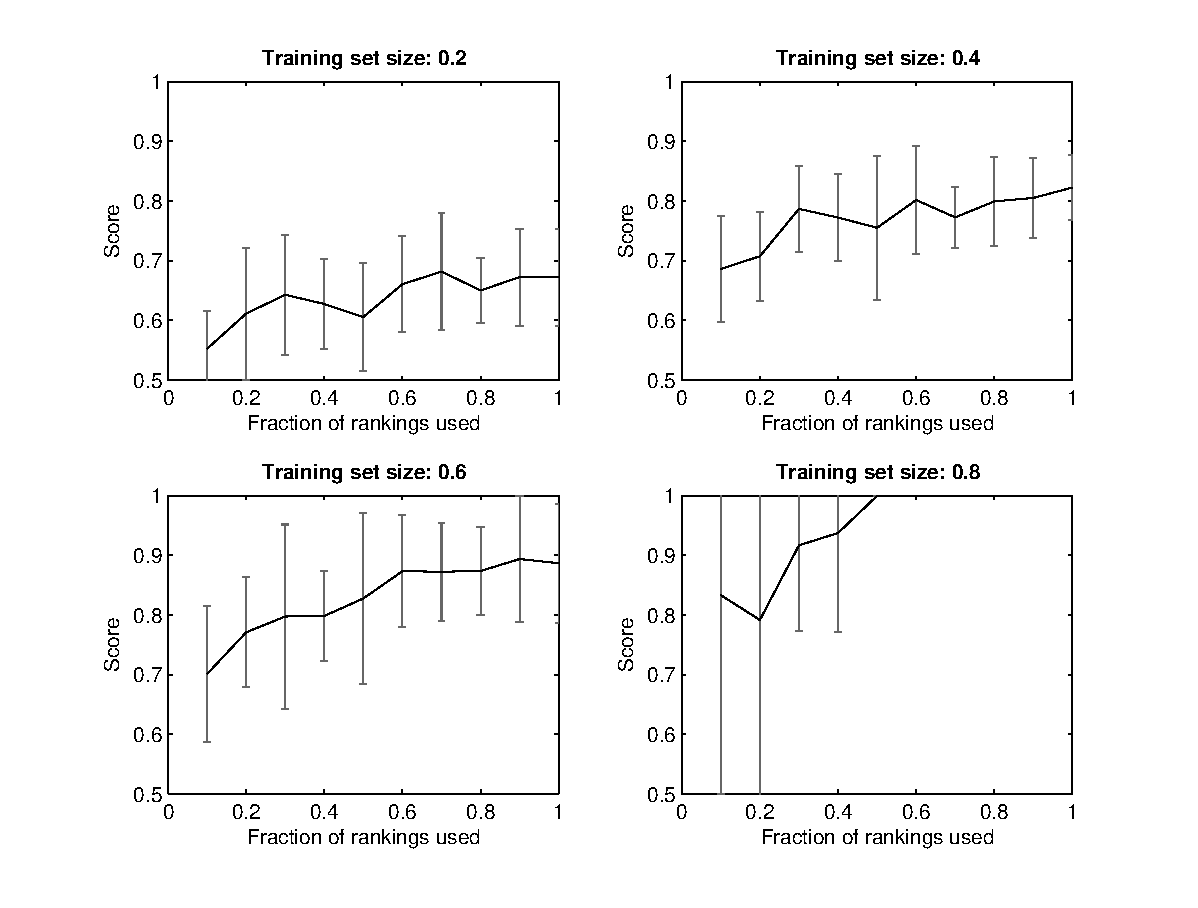
\includegraphics[width=1\linewidth]{rankings}
  \caption{Invloed fractie ongelijkheden}
  \label{fig:fractie}

\end{figure}

Figuur~\ref{fig:fractie} toont aan dat de scores voor grotere leersets en meer beschikbare ongelijkheden toeneemt.
Hierbij worden steeds meer dan 50\% van de paren juist voorspeld en worden redelijk hoge scores behaald zelfs voor kleiner leersets.
Andere experimenten hebben laten zien dat zelfs voor lagere scores de optimalisatie criteria in staat zijn de optimale oplossing te bepalen.
Gelijkaardige scores worden behaald indien het achterliggende model clausules gebruikt die niet door het leersysteem gegenereerd kunnen worden.

\begin{figure}

  \centering
    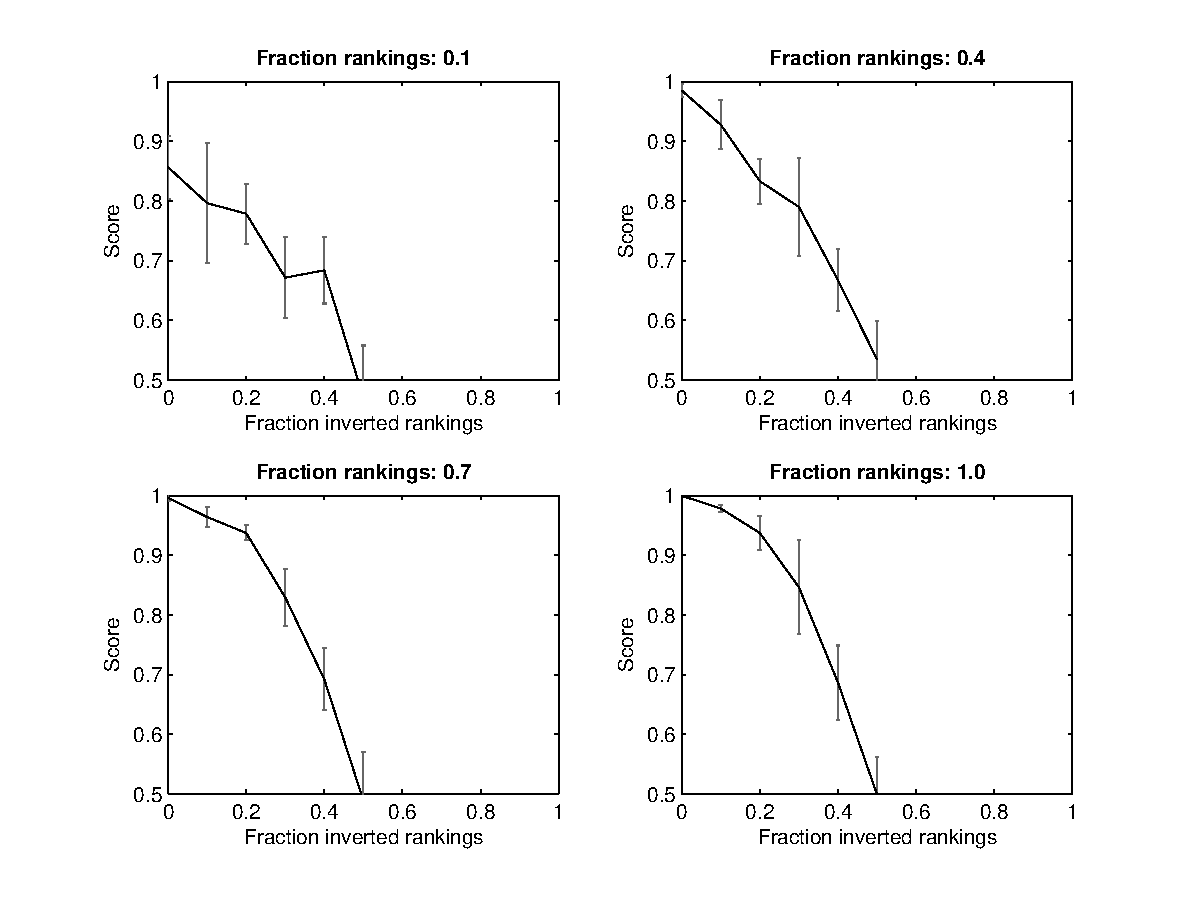
\includegraphics[width=1\linewidth]{noise}
  \caption{Invloed ruis}
  \label{fig:ruis}

\end{figure}

In figuur~\ref{fig:ruis} wordt de invloed van ruis getoond indien alle voorbeelden beschikbaar zijn voor het leren van de zwakke beperkingen.
Het algoritme blijkt bestand te zijn tegen redelijke percentages aan foute rangschikkingen.
Ook bij het gebruik van een leerset met 40\% van de voorbeelden kunnen redelijke scores boven 0.7 behaald worden als 20\% van de rangschikkingen fout zijn.

  \begin{table}
    \caption{Scores voor verschillende limieten ($t$)}
    \begin{tabularx}{\linewidth}{XXXX}
      $t = 1$ & $t = 2$ & $t = 3$ & $t = 4$ \\
      \toprule
     0.823 & 0.740 & 0.788 & 0.735 \\
     ($\pm$ 0.073)&
($\pm$ 0.078)&
($\pm$ 0.074)&
($\pm$ 0.063)
    \end{tabularx}
    \label{tbl:limiet}
  \end{table}

Uiteindelijk toont tabel~\ref{tbl:limiet} dat het verhogen van de limiet voor het vinden van zachte beperkingen de score niet verhoogt.
Het experiment gebruikt een leerset van 40\% en 40\% van de beschikbare ongelijkheden.
Het is wel denkbaar dat voor grotere voorbeelden een hogere limiet wenselijk is.

% An example of a floating figure using the graphicx package.
% Note that \label must occur AFTER (or within) \caption.
% For figures, \caption should occur after the \includegraphics.
% Note that IEEEtran v1.7 and later has special internal code that
% is designed to preserve the operation of \label within \caption
% even when the captionsoff option is in effect. However, because
% of issues like this, it may be the safest practice to put all your
% \label just after \caption rather than within \caption{}.
%
% Reminder: the "draftcls" or "draftclsnofoot", not "draft", class
% option should be used if it is desired that the figures are to be
% displayed while in draft mode.
%
%\begin{figure}[!t]
%\centering
%\includegraphics[width=2.5in]{myfigure}
% where an .eps filename suffix will be assumed under latex, 
% and a .pdf suffix will be assumed for pdflatex; or what has been declared
% via \DeclareGraphicsExtensions.
%\caption{Simulation results for the network.}
%\label{fig_sim}
%\end{figure}

% Note that IEEE typically puts floats only at the top, even when this
% results in a large percentage of a column being occupied by floats.


% An example of a double column floating figure using two subfigures.
% (The subfig.sty package must be loaded for this to work.)
% The subfigure \label commands are set within each subfloat command,
% and the \label for the overall figure must come after \caption.
% \hfil is used as a separator to get equal spacing.
% Watch out that the combined width of all the subfigures on a 
% line do not exceed the text width or a line break will occur.
%
%\begin{figure*}[!t]
%\centering
%\subfloat[Case I]{\includegraphics[width=2.5in]{box}%
%\label{fig_first_case}}
%\hfil
%\subfloat[Case II]{\includegraphics[width=2.5in]{box}%
%\label{fig_second_case}}
%\caption{Simulation results for the network.}
%\label{fig_sim}
%\end{figure*}
%
% Note that often IEEE papers with subfigures do not employ subfigure
% captions (using the optional argument to \subfloat[]), but instead will
% reference/describe all of them (a), (b), etc., within the main caption.
% Be aware that for subfig.sty to generate the (a), (b), etc., subfigure
% labels, the optional argument to \subfloat must be present. If a
% subcaption is not desired, just leave its contents blank,
% e.g., \subfloat[].


% An example of a floating table. Note that, for IEEE style tables, the
% \caption command should come BEFORE the table and, given that table
% captions serve much like titles, are usually capitalized except for words
% such as a, an, and, as, at, but, by, for, in, nor, of, on, or, the, to
% and up, which are usually not capitalized unless they are the first or
% last word of the caption. Table text will default to \footnotesize as
% IEEE normally uses this smaller font for tables.
% The \label must come after \caption as always.
%
%\begin{table}[!t]
%% increase table row spacing, adjust to taste
%\renewcommand{\arraystretch}{1.3}
% if using array.sty, it might be a good idea to tweak the value of
% \extrarowheight as needed to properly center the text within the cells
%\caption{An Example of a Table}
%\label{table_example}
%\centering
%% Some packages, such as MDW tools, offer better commands for making tables
%% than the plain LaTeX2e tabular which is used here.
%\begin{tabular}{|c||c|}
%\hline
%One & Two\\
%\hline
%Three & Four\\
%\hline
%\end{tabular}
%\end{table}


% Note that the IEEE does not put floats in the very first column
% - or typically anywhere on the first page for that matter. Also,
% in-text middle ("here") positioning is typically not used, but it
% is allowed and encouraged for Computer Society conferences (but
% not Computer Society journals). Most IEEE journals/conferences use
% top floats exclusively. 
% Note that, LaTeX2e, unlike IEEE journals/conferences, places
% footnotes above bottom floats. This can be corrected via the
% \fnbelowfloat command of the stfloats package.




\section{Conclusie}
In dit onderzoek werden leersystemen voor beperkingen en optimalisatie criteria ontworpen.
Hiermee konden de vooropgestelde doelstellingen bereikt worden.

Het leersysteem voor beperkingen kon zowel de harde als de zachte beperkingen leren voor alle onderzochte problemen.
Hiermee is het eerste doel van dit onderzoek bereikt.
De problemen konden allemaal opgelost worden in beperkte tijd (minder dan een minuut) en vaak in enkele seconden.
Er werden telkens maar weinig voorbeelden gebruikt om van te leren.
Het systeem stelt minimale eisen aan de gebruiker maar laat toe om expressieve achtergrondkennis te voorzien.
De geleerde beperkingen zijn onafhankelijk van een specifiek domein, dit vergemakkelijkt het opstellen van positieve voorbeelden.

Ook aan het tweede doel van deze thesis, het leren van optimalisatie beperkingen, werd voldaan.
Het leersysteem voor optimalisatie beperkingen kon gewogen beperkingen vinden die toelaten op optimale oplossingen te vinden.
Zelfs bij kleine datasets en ruis op de onderliggende preferenties konden beperkingen gevonden worden waarmee de meeste voorbeelden correct gerangschikt worden.

Naast het faciliteren van het automatische leren van formele representaties kon ook worden uitgewerkt hoe deze representaties kunnen gebruikt worden om (optimale) oplossingen te vinden.
Daarmee is ook een belangrijke stap gezet om interactieve varianten mogelijk maken voor het opstellen van (gewogen) clausules in eerste orde logica. 

\paragraph{Toekomstig werk}
Dit onderzoek biedt veel aanknopingsmogelijkheden.
Het zou interessant zijn om het aantal variabelen en literalen in een clausule dynamisch aan te passen.
Hiertoe kunnen bijvoorbeeld negatieve voorbeelden gebruikt worden.
Door te bepalen wanneer geen negatief voorbeeld meer aanvaard wordt kan het algoritme zelf stoppen.

Het toevoegen van interactiviteit zou de leersystemen kunnen verbeteren, zowel door het genereren van voorbeelden als het vragen om rangschikkingen.
Rangschikkingen kunnen meerdere voorbeelden bevatten, maar gelijkheden worden op dit moment genegeerd.
Nochtans bevatten deze belangrijke informatie, indien een gebruiker deze expliciet opgeeft.

Het feit dat de geleerde clausules onafhankelijk zijn van de specifieke voorbeelden heeft verschillende voordelen.
In sommige gevallen zijn er echter specifieke objecten die eigen zijn aan het probleem zelf.
Het leersysteem zou kunnen uitgebreid worden om globale constanten, die onafhankelijk zijn van specifieke voorbeelden, te ondersteunen. 

% conference papers do not normally have an appendix


% use section* for acknowledgment
\section*{Dankwoord}
De auteur bedankt zijn promotoren Prof. dr. Luc De Raedt en Dr. ir. Anton Dries.
Bovendien is hij dankbaar voor de hulp van Bart Bogaerts, Prof. dr. Jesse Davis, Prof. dr. Marc Denecker en Vladimir Dzyuba.

% trigger a \newpage just before the given reference
% number - used to balance the columns on the last page
% adjust value as needed - may need to be readjusted if
% the document is modified later
%\IEEEtriggeratref{8}
% The "triggered" command can be changed if desired:
%\IEEEtriggercmd{\enlargethispage{-5in}}

% references section

% can use a bibliography generated by BibTeX as a .bbl file
% BibTeX documentation can be easily obtained at:
% http://www.ctan.org/tex-archive/biblio/bibtex/contrib/doc/
% The IEEEtran BibTeX style support page is at:
% http://www.michaelshell.org/tex/ieeetran/bibtex/
%\bibliographystyle{IEEEtran}
% argument is your BibTeX string definitions and bibliography database(s)
%\bibliography{IEEEabrv,../bib/paper}
%
% <OR> manually copy in the resultant .bbl file
% set second argument of \begin to the number of references
% (used to reserve space for the reference number labels box)

\bibliographystyle{abbrv}
\bibliography{Bibliography.bib}


% that's all folks
\end{document}


